

\section{Definition of simulation scenarios} \label{sec:definition_of_simulation_scenarios}

In this section the simulation scenarios and settings are described to get a complete picture of the simulated cloud environment. 

The simulation scenarios can be divided into two parts which are day ahead and real time simulations based on day ahead and real time energy prices, respectively. For each type of simulation different locations and energy markets have been chosen. The basic scenario types are oulined below. 


\subsection{Day ahead simulation scenario}

The simulation scenario for day ahead energy prices is comprised of data centers located in Europe and the USA. A map showing five data centers as a basis for day ahead simulations is outlined in Figure \ref{fig:usa_europe_map}. 

\begin{figure}[htbp]
	\centering
		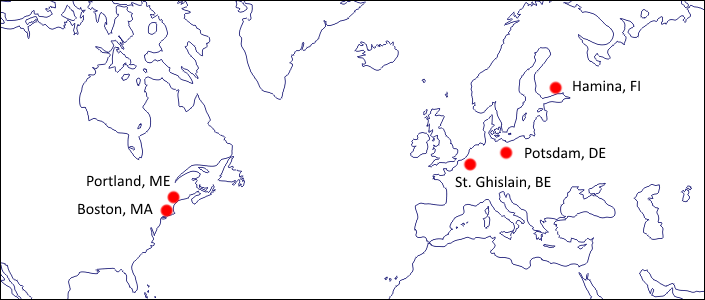
\includegraphics[width=0.7\textwidth]{figures/evaluation_and_results/usa_europe_map.png}
	\caption{Map of data center locations for day ahead price simulations}
	\label{fig:usa_europe_map}
\end{figure}

The locations have been chosen such that a diverse set of data from different energy markets is available. In addition time zone effects should be modeled by placing data centers sufficiently far from each other such that daily variation of energy prices in different time zones can be utilized. 

A list of day ahead energy markets and corresponding locations is shown in Table \ref{tab:list_of_day_ahead_markets}. 


\begin{table}[htbp]
\centering
\begin{tabular}{ll}
\toprule
 Energy market & Location \\
\midrule
	Nord Pool Spot &  Hamina, Finland \\
	Belpex &  St. Ghislain, Belgium \\
	EPEXSpot &  Potsdam, Germany \\
	ISO New England &  Portland, Maine \\
	ISO New England &  Boston, Massachussetts \\
\bottomrule
\end{tabular}
\caption{List of day ahead energy markets and locations}
\label{tab:list_of_day_ahead_markets}
\end{table}




\subsection{Real time simulation scenario}

For the real time simulation scenario data centers have been chosen exclusively from location within the US. Thus energy prices are more localized and performance of simulations should be evaluated for datasets with similar characteristics in contrast to day ahead simulations. 

A map showing data centers for all real time markets and locations is depicted in Figure \ref{fig:usa_map}. 

\begin{figure}[htbp]
	\centering
		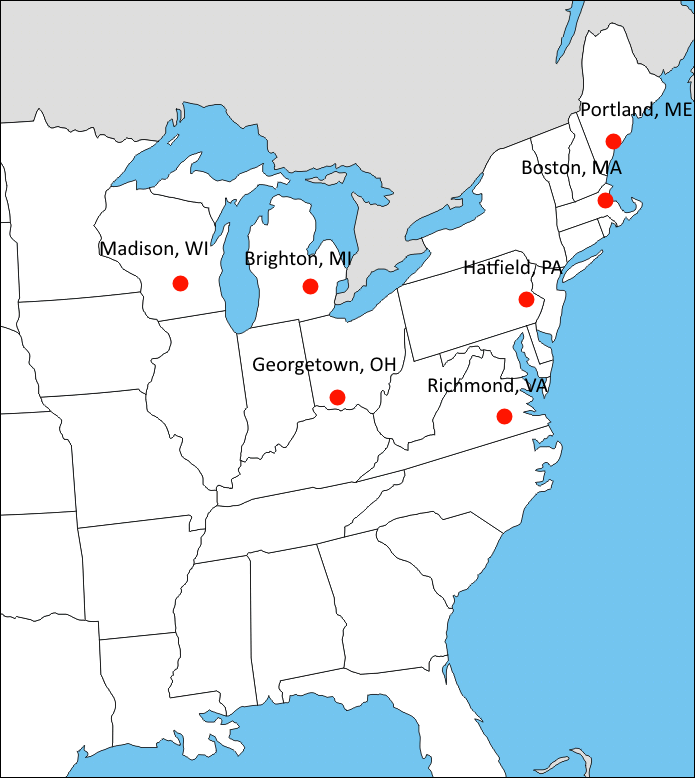
\includegraphics[width=0.50\textwidth]{figures/evaluation_and_results/usa_map.png}
	\caption{Map of data center locations for real time price simulations}
	\label{fig:usa_map}
\end{figure}

A list of real time energy markets and locations is outlined in Table \ref{tab:list_of_real_time_markets}. 

\begin{table}[htbp]
\centering
\begin{tabular}{ll}
\toprule
 Energy market & Location \\
\midrule
	ISO New England &  Portland, Maine \\
	ISO New England &  Boston, Massachussetts \\
	PJM & Richmond, Virginia  \\
	PJM & Brighton, Michigan  \\
	PJM & Hatfield, Pennsylvania  \\
	PJM & Madison, Wisconsin  \\
	PJM & Georgetown, Ohio  \\
\bottomrule
\end{tabular}
\caption{List of real time energy markets and locations}
\label{tab:list_of_real_time_markets}
\end{table}





\subsection{Simulation Configuration Parameters} \label{ssec:simulation_configuration_parameters}

\subsubsection{Cloud settings}

As the simulator has been built to be highly configurable \cite{lucanin2015philharmonic} different cloud parameters can be adjusted to run simulations with different settings. In Table \ref{tab:list_of_cloud_metrics} the most relevant simulation parameters are listed. 

\begin{table}[htbp]
\centering
\begin{tabularx}{\textwidth}{l|l|X}
	Metric & Values & Description \\
\hline
	number of servers & 500 & The total number of servers across all locations \\
	number of virtual machines & 5000 & The total number of virtual machines over the whole simulation time period \\
	server cpus & $[4,8]$ & The number of CPUs per server uniformly distributed over the given interval \\
	server memory & $[8,16]$ & The amount of memory per server uniformly distributed over the given interval \\
	virtual machine cpus & $[1,4]$ & The number of CPUs per VM uniformly distributed over the given interval \\
	virtual machine memory & $[1,4]$ & The amount of memory per VM uniformly distributed over the given interval \\
	dirty page rate & $\{20,40,70,90\}$ & One of four dirty page rates in MB/s assigned to each VM \\
	SLA level & 99.95\% & A fixed SLA availability level applied to each VM \\
	VM duration & $\{1,2,5,8,12,24,48\}$ & A fixed set of duration values in hours applied uniformly to the set of VMs \\
	VM price & 4 \cent \ / h & The price of a VM in cent per hour \\
	bandwidth & $\{400,800,1000\}$ & One of 3 amounts of bandwidths in MBit/s set between each two locations \\
	bandwidth cost & 0.1 \cent \ / GB & Bandwidth costs in cent per GB \\
	server peak power & 200 W & The power a server draws when its resources are fully utilized \\
	server idle power & 100 W & The power a server draws when idle \\
	cpu resource weight & 0.7 & The weight associated with cpu power when calculating server utilization \\
	memory resource weight & 0.3 & The weight associated with memory when calculating server utilization \\
\end{tabularx}
\caption{List of cloud configuration parameters in the simulation}
\label{tab:list_of_cloud_metrics}
\end{table}

The number of servers and VMs per simulation has been adjusted such that the resulting utilization is reasonable, e.g.~with 1000 servers and 2000 VMs in total an average utilization of only about 1 \% has been achieved over a simulation period of 5 weeks. Thus raising the number of VMs and in turn reducing number of servers led to a more realistic utilization of 30\% to 40\%. 

The relation of number of resources per server to the amount of VM resources (i.e.~number of cpus, memory) has been defined such that capacity constraints will not be an issue in simulations. The same method has been applied to the relation of total number of servers to number of VMs. 

The dirty page rate has a direct impact on VM migration performance (see Section \ref{sec:modeling_migration_energy}) and therefore different values have been assigned to VMs to simulate different application behavior. In combination with bandwidth this may lead to a high variation in migration downtimes. 

The SLA level has been set to the most common value for internet cloud services \cite{google2015compute,amazon2013sla}. With different penalty levels greater downtimes directly impact resulting costs for cloud providers. 

A different set of duration values has been assigned to VMs in order to simulate different kinds of workloads. This includes VM durations of 1 to 48 hours for scientific or HPC applications. Long running VMs have been omitted to focus on short term applications. 

The VM price most resembles the price for a ``n1-standard-1'' VM on Google Compute Cloud\footnote{\url{https://cloud.google.com/compute/pricing}}. As this is one of the smallest VMs available in the Google Cloud this price is still comparably cheap. 

Bandwidth is divided into low, medium and high values to simulate real world scenarios where high bandwidth may not always be available. As bandwidth has a direct impact on migration downtime this allows to evaluate the total resulting downtime and costs in different scenarios. 

Bandwidth costs have been set to a fixed price per amount of traffic while it is usually paid by fixed price contracts with 95/5 bandwidth constraints \cite{qureshi2009cutting}. These contracts measure traffic in fixed time intervals and the 95-th percentile of total usage is charged. To simplify the model in this work it has been set to a fixed price per volume. 

Server peak and idle power have been set where a server at peak load consumes double the amount of power than when idle. This may be too optimistic as it is stated that servers consume about 60\% of power when idle \cite{meisner2009powernap}. However studies show that new server technology is able to achieve power reductions up to 75\% from peak to idle mode \cite{prime2011energy}. 
A greater ratio of peak to idle power results in greater possibility for energy savings. Therefore the idle-to-peak ratio is critical for any scheduling algorithms aiming to reduce costs based on energy. 

CPU and memory resource weights have been defined to calculate resulting power consumption from server utilization of each resource. From investigations in \cite{meisner2009powernap,kansal2010virtual} it can be deduced that CPU is the most power consuming component where memory power consumption amounts to about one third up to equal amounts of CPU power. Therefore CPU and memory weights have been set to accommodate those findings. 



\subsubsection{Cloud scheduler} \label{sec:cloud_scheduler}

The core of the simulation is represented by the Cloud Scheduler. It is responsible for managing requests and for deciding which VMs should be migrated at which point in time. To make it a flexibel approach and be able to compare different scenarios the scheduler can be configured to run one out of seven different scenarios (Table \ref{tab:existing_scheduling_scenarios}). 


\begin{table}[htbp]
\centering
\begin{tabular}{lll}
\hline
  & \textbf{Request assignment} & \textbf{Migration handling} \\
\hline
	BFD baseline scheduler &  not cost aware, based on load & None \\
	BCF scheduler & cost aware, no forecasts & None \\
	BCF scheduler + FC & cost aware, forecasts & None \\
	BCF scheduler + Ideal FC & cost aware, ideal forecasts & None \\
	BCU scheduler + M & cost aware, no forecasts & cost aware, no forecasts \\
	BCU scheduler + M + FC & cost aware, forecasts & cost aware, forecasts \\
	BCU scheduler + M + ideal FC & cost aware, ideal forecasts & cost aware, ideal forecasts \\
\hline
\end{tabular}
\caption{Existing scheduling scenarios}
\label{tab:existing_scheduling_scenarios}
\end{table}

The first scheduler is a \textit{Best Fit Decreasing} (BFD) Scheduler that does no investigations on energy prices at all. It is based on a load balancing approach which aims to assign requests to the least occupied data center and utilize as few servers as possible to save energy costs. The BFD Scheduler is outlined in algorithm \ref{alg:bfd_scheduler}. 

The BFD scheduler iterates over the set of VM requests at the current point in time and aims to optimize placement of VMs by considering resource utilization of VMs and PMs for maximum consolidation. VM requests are sorted by resources in descending order to process VMs exhibiting large resource requirements first (line2). Locations are sorted by utilization ascending to assign requests first to under utilized locations (line 3). Lines 4 and 5 denote sorting of PMs by (free) capacities to consider most occupied servers first. 

\begin{algorithm}[htpb]
	\SetAlgoLined
	\SetKwProg{Fn}{Function}{:}{}
	\Fn{BFD Scheduler}{
		\KwData{Input Requests}
		\KwResult{Requests assigned according to BFD Schedule}
		sort VM requests with resource utilization in descending order\;
		sort locations by utilization in ascending order\;
		sort available PMs by location and free capacities in ascending order\;
		sort inactive PMs by capacities in ascending order\;
		
		\ForEach{vm in VM requests}{
			\While{vm not assigned {\normalfont and} size(available PMs) > 0}{
				\ForEach{pm in available PMs}{
					\If{vm fits on pm}{
						assign vm to pm\;
						remove vm from available PMs\;
						break\;
					}
				}
				
				\eIf{vm not assigned {\normalfont and} size(inactive PMs) > 0}{
					add first of inactive PMs to available PMs\;
					sort available PMs by location and free capacities ascending\;
				}{
					break\;
				}			
			}
		}
	}
\caption{Best fit decreasing scheduler}
\label{alg:bfd_scheduler}
\end{algorithm}

The BFD algorithm iterates over the set of requests and tries to assign VMs to hosts as long as non-fully occupied servers are available (line 7,8-14). In case a VM could not be assigned a server from the set of inactive hosts is activated and the aforementioned procedure is executed again (lines 15-17). In case no suitable host could be found or no further hosts are available the loop is exited with the current VM not being assigned (lines 18-19). 

As discussed before Table \ref{tab:existing_scheduling_scenarios} describes further scenarios with different scheduling algorithms. 
These algorithms are based on the \textit{Best Cost Fit} (BCF) and \textit{Best Cost Utility} (BCU) Scheduler with different variations to include migrations (denoted by \textit{M}), forecasts (denoted by \textit{FC}) and ideal forecasts (denoted by \textit{ideal FC}). 

The next discussed algorithm is the one from the Best Cost Fit scheduler which aims to maximize cost savings when assigning requests utilizing price forecasts. The corresponding algorithm is outlined in \ref{alg:bcf_scheduler}. 

\begin{algorithm}[htpb]
	\SetAlgoLined
	\SetKwProg{Fn}{Function}{:}{}
	\Fn{BCF Scheduler}{
		\SetKwInOut{Input}{Data}
    \SetKwInOut{Output}{Result}
		\Input{Input Requests \\
						flag for forecasts (FC)\\
						flag for ideal FC (idealFC)}
		\KwResult{Requests assigned according to BCF Schedule and given scenario}
		sort VM requests with resource utilization in descending order\;
		
		maxH <- 1\;
		\If{FC}{maxH <- get max fc horizon from config\;}
		
		\ForEach{vm in VM requests}{
			dur <- get remaining duration for vm\;
			\eIf{dur <= 1}
			{FC <- false\;idealFC <- false\;}
			{maxH <- min(dur,maxH)\;}
			
			fcData <- get sorted price and forecast data (FC, idealFC)\;
		
			\ForEach{data in fcData}{
				h <- get forecast horizon (data)\;
				loc <- get location (data)\;
				assign to host BFD (vm, loc)\;
				\If{assigned}{
					block vm for the next h time periods\;
					break\;
				}
			}
		}
	}
\caption{Best cost fit scheduler}
\label{alg:bcf_scheduler}
\end{algorithm}


The best cost fit scheduler takes three inputs: The VM requests, a flag denoting whether forecasts should be enabled and a second flag for possible inclusion of ideal forecasts. In line 2 requests are sorted descending by their resource requirements which resembles the step in the BFD scheduler. 

Lines 3-6 determine the maximum forecast horizon that should be taken into account when considering future energy prices (in case forecasts are enabled). From lines 7-11 the set of VM requests is iterated and forecasts are enabled based on the remaining duration. Line 13 determines the forecast horizon that will be applied through a minimum function of the remaining VM duration and the maximum forecast horizon defined previously. 

In line 15 a procedure is called to retrieve locations and best estimated forecast windows for these locations. Thus for each location and forecast horizon the average estimated energy price is calculated and results are sorted by price ascending such that the location with the least expected costs regarding a specific forecast horizon is placed first. 

\begin{algorithm}[htpb]
	\SetAlgoLined
	\SetKwProg{Fn}{Function}{:}{}
	\Fn{BCU Scheduler}{
		\SetKwInOut{Input}{Data}
    \SetKwInOut{Output}{Result}
		\Input{Input Requests \\
						Current cloud state \\
						flag for forecasts (FC)\\
						flag for ideal FC (idealFC)}
		\KwResult{A list of VMs with resulting utility value above the utility threshold}
		[slaPen,migEnergy,maxMigEnergy,remDur,maxRemDur,util,estimatedSavings] <- prepare utility function (FC, idealFC)\;
		
		uResult <- []\;
			
		\ForEach{vm in VM requests}{
		
			currentLoc <- getLocation(vm)\;
			uValue <- []\;
		
			\ForEach{loc in locations}{
				\If{loc != currentLoc}{
					
					slaPenalty <- 1 - slaPen[vm][loc]\;
					migrationEnergy <- 1 - (migEnergy[vm][loc] / maxMigEnergy)\;
					remainingDur <- remDur[vm] / maxRemDur\;
					dcLoad <- getRelativeDCLoad (util, currentLoc)\;
					costSavings <- estimatedSavings[vm][loc]\;
					
					result <- wSLA * slaPenalty + wMig * migrationEnergy + wDur * remainingDur + wLoad * dcLoad + wCost * costSavings\;
					
					uValue [loc] <- result\;
				}	
			}
			
			maxUValue <- max(uValue)\;
			append (uResult, (vm, getLocation(maxUValue), getUtilityValue(maxUValue)))\;
		}
		
		sort uResult by utility value descending\;
		result <- []\;
		uTH <- get utility TH from config ()\;
		
		\ForEach{r in uResult}{
			\If{utilityValue(r) > uTH}{
				append (result, r)\;
			}
		}
		
		return result\;
	}
\caption{Best cost utility scheduler}
\label{alg:bcu_scheduler}
\end{algorithm}

In lines 16 to 24 the resulting dataset from line 15 is iterated and the forecast horizon and location from the cheapest to more expensive locations are retrieved. For each of these data it is tried to assign the VM to a host from the given location based on a BFD approach. If the VM could be assigned successfully the VM will be blocked for migrations for the next $h$ time periods to prevent oscillation of VMs between different locations. 

The last scheduler is the Best Cost Utility Scheduler that takes into account VM migrations between different locations based on a utility function (see Section \ref{ssec:cloud_scheduler_and_utility_function} for a definition of the utility function). 
The algorithm of the BCU scheduler is shown in \ref{alg:bcu_scheduler}. 

Line 2 of the algorithm calls the procedure \textit{prepare utility function} that returns a list of metrics depending on the flags \textit{FC} and \textit{idealFC}. Results of utility calculations are stored in \textit{uResult} in line 3. 

From lines 4-6 start iterating over the set of VM requests and prepare the current location and a list of utility values. In addition lines 7 and 8 start iterating over the set of locations where the current location is skipped for migration. From line 9 to 13 the different criteria values are normalized from the results of the procedure in line 2. A list of criteria regarding this utility function can be found in Section \ref{ssec:cloud_scheduler_and_utility_function}. 

In line 14 the total utility value is calculated where each normalized criteria is weighted with its corresponding weight. The total utility value  is stored in line 15 for the current VM \textit{vm} and location \textit{loc}. Line 18 calculates the maximum utility value for this VM over all locations. That is, the most promising location where VM \textit{vm} could be migrated to is estimated. 

In line 19 a tuple consisting of \textit{(vm, loc, uvalue)} is added to the result utility list where \textit{uvalue} is the maximum of the calculated utility values for VM \textit{vm} associated with location \textit{loc}. 
Line 21 sorts the result utility list by utility value descending and line 22 and 23 are preparing the final result list and the utility threshold, which is taken from a configuration file. 

Lines 24 to 28 iterate over the resulting utility list and add values to the final result list in case the corresponding utility value exceeds the predefined utility threshold \textit{uTH}. 
The algorithm is concluded by returning the list of result VMs with total utility values above the utility threshold in line 29. 



\subsection{Cost models}

Cost models and related metrics are an important base for transforming aggregated power values to actual costs. Therefore a number of formulas have been defined to accurately model the resulting power consumption and energy costs. 
%These formulas are outlined below. 

\paragraph{Utilization of servers}
The basis for modeling power consumption is to define resource utilization of servers since server utilization relates directly to resulting power consumption \cite{meisner2009powernap}. 
Server utilization based on a set of resources $R$ is defined in Equation \ref{eq:server_utilization}. 

\begin{equation}
	s_{util}(t) = \sum_{r \in R} w_r \frac{s_{used}(r,t)}{s_{cap}(r)}
	\label{eq:server_utilization}
\end{equation}

with $w_r$ denoting the weight of resource $r$, $s_{used}$ is the currently used capacity of server $s$ regarding resource $r$ at time $t$, $s_{cap}$ denotes the total capacity of server $s$ of resource $r$ and $s_{util}$ being the resulting utilization of the server. 


\paragraph{Utilization per location}
In order to calculate data center load for each location a method of computing the average utilization per location is needed. 
It is defined as the average utilization of all servers in a given location (Equation \ref{eq:utilization_per_location}): 

\begin{equation}
	util_{loc}(t) = \frac{1}{|loc_{s}|} \sum_{s \in loc_{s}} s_{util}(t)
\label{eq:utilization_per_location}
\end{equation}

where $loc_{s}$ being the set of servers at location $loc$ and $util_{loc}$ denotes the current utilization at location $loc$. 


\paragraph{Power per location}

From the previous metric \textit{utilization per location} the resulting cloud power per location can be derived (Equation \ref{eq:power_loc}). 

\begin{equation}
	power_{loc}(t) = util_{loc}(t) \cdot |loc_{active_s}(t)| \cdot (P_{peak} - P_{idle}) + |loc_{active_s}(t)| \cdot P_{idle}
\label{eq:power_loc}
\end{equation}

where $|loc_{active_s}(t)|$ is the number of active servers at location $loc$ at time $t$, $P_{peak}$ is the peak power of the server and $P_{idle}$ describes the idle power of the server. 

\paragraph{Total cloud power}

The total cloud power is the sum of power consumption over all locations $L$ and time periods $T$ (Equation \ref{eq:m_tcp}). 

\begin{equation}
	m_{TCP} = \sum_{t \in T} \sum_{loc \in L} power_{loc}(t)
\label{eq:m_tcp}
\end{equation}


\paragraph{Migration load}
This metric serves as the basis for calculating migration energy as it directly depends on migration load. In addition it is used for further metrics such as migration costs. The formula for aggregated migration load per time $t$ is outlined in Equation \ref{eq:migration_load}.

\begin{equation}
	mig_l(t) = \sum_{v \in VM} V_{mig}(v,t)
\label{eq:migration_load}
\end{equation}

where $VM$ denotes the set of all active VMs at time $t$ and $V_{mig}(v,t)$ is the total migration load for vm $v$ for a migration starting at time $t$. The latter expression is taken from the definition of migration energy in Section \ref{sec:modeling_migration_energy}. 

\paragraph{Migration energy}
Modeling migration energy is needed for calculating the migration costs and it may also give a hint for resulting downtime and possible penalty costs due to the amount of migration energy consumed. 
The formulas for summed migration energy over the set of all VMs $VM$ and total migration energy over a simulation time period are denoted in Equations \ref{eq:migration_energy_by_time} and \ref{eq:migration_energy_total}. 

\begin{align}
	mig_e(t) = \sum_{v \in VM} E_{mig}(v,t) \label{eq:migration_energy_by_time}\\
	m_{ME} = \sum_{t \in T} mig_e(t) \label{eq:migration_energy_total}
\end{align}

\paragraph{Migration cost}
The migration costs are defined on the one side by combining resulting migration energy with current energy prices and on the other side by combining migration load and bandwidth costs. 

\begin{align}
	p_{mean}(t) &= \frac{p_{l1}(t) + p_{l2}(t)}{2} \label{eq:p_mean} \\
	mig_c(t) &= mig_e(t) \cdot p_{mean}(t) \label{eq:mig_c} \\
	mig_{c_{bw}}(t) &= mig_l(t) \cdot c_{bw} \label{eq:mig_c_bw} \\
	m_{MC} &= \sum_{t \in T} \left( mig_c(t) + mig_{c_{bw}}(t) \right) \label{eq:m_mc} 
\end{align}

Equation \ref{eq:p_mean} shows the mean price calculated from prices $p_{l1}$ and $p_{l2}$ in locations $l1$ and $l2$ at time $t$. 
Equation \ref{eq:mig_c} describes the migration costs depending on the migration energy and mean energy price $p_{mean}$ at time $t$. 
The bandwidth related costs for migration are outlined in Equation \ref{eq:mig_c_bw} with migration load and bandwidth costs combined (i.e.~amount of GB multiplied by \cent \ / GB). The migration cost metric $m_{MC}$ in Equation \ref{eq:m_mc} is then the sum of both energy and bandwidth costs. 

\paragraph{Cost of VM}
The resulting costs $v_c$ for a user of a VM is defined as the price $v_p$ set for the VM multiplied by its duration up to time $t$ (Equation \ref{eq:cost_of_vm}). 

\begin{equation}
	v_c(t) = v_p \cdot v_{dur}(t)
\label{eq:cost_of_vm}
\end{equation}

\paragraph{Penalty cost}

The total penalty costs are the aggregated costs for all penalties and VMs occurred during a simulation. Penalty costs occur when the maximum allowed downtime for a VM regarding an SLA threshold is exceeded. Depending on the threshold that has been surpassed different penalty costs have to be paid. 
As described in Section \ref{sec:sla_managemenet} three different penalty thresholds are defined which result in different penalty costs. 

\begin{align}
	SLA_{TH_i}(v,t) &= v_{dur}(t) \left( 1 - \frac{v_{SLA_i}}{100} \right), i \in \{1,2,3\} \label{eq:sla_th_i} \\
	v_{SLA_1} &= 99.95, v_{SLA_2} = 99, v_{SLA_3} = 95 \label{eq:sla_levels} \\
	v_{pen}(t) &= \left\{
								\begin{array}{@{}ll@{}}
									0.5, & \text{if } down_{acc}(v,t) > SLA_{TH_3}(v,t) \\
									0.25, & \text{if } down_{acc}(v,t) > SLA_{TH_2}(v,t) \\
									0.1, & \text{if } down_{acc}(v,t) > SLA_{TH_1}(v,t) \\
									0, & \text{otherwise}
								\end{array}\right. \label{eq:v_pen}  \\
	v_{c_{pen}}(t) &= v_c(t) \cdot v_{pen}(t) \label{eq:v_c_pen} \\
	m_{TPC} &= \sum_{v \in VM} v_{c_{pen}}(t_{last}) \label{eq:m_pc} 
\end{align}

Equation \ref{eq:sla_th_i} defines an SLA threshold for either of the defined SLA levels in Equation \ref{eq:sla_levels}. In Equation \ref{eq:v_pen} penalty values in the interval [0,1] are assigned based on the SLA threshold reached. This penalty value is then applied to the costs of the VM in Equation \ref{eq:v_c_pen} resulting in penalty costs for VM $v$. Equation \ref{eq:m_pc} calculates the total penalty costs across all VMs at the last simulation time stamp $t_{last}$. 


\paragraph{Total downtime}

The total downtime is calculated from the sum of downtimes of all VMs over the whole simulation time period (up to $t_{last}$, Equation \ref{eq:m_tdt}). 

\begin{equation}
	m_{TDT} = \sum_{v \in VM} down_{acc}(v,t_{last})
\label{eq:m_tdt}
\end{equation}

\paragraph{Number of migrations}

The total number of migrations is defined as the sum of migrations at each time stamp $t$ (Equation \ref{eq:num_migrations}). 

\begin{equation}
	m_{NM} = \sum_{t \in T} mig_{num} (t) 
\label{eq:num_migrations}
\end{equation}

where $mig_{num}(t)$ denotes the number of migrations at time $t$. 


\paragraph{Total cloud costs}

The total cloud costs are calculated as the sum of cloud power values multiplied by the price at the respective location and time (Equation \ref{eq:m_tcc}). 

\begin{equation}
	m_{TCC} = \sum_{t \in T} \sum_{loc \in L } power_{loc}(t) \cdot p_{loc}(t)
\label{eq:m_tcc}
\end{equation}

\paragraph{Total cloud power with migrations}

Calculating the total cloud power including migrations is a simple addition of the total cloud power and migration energy (Equation \ref{eq:m_tcpwm}). 

\begin{equation}
	m_{TCPWM} = m_{TCP} + m_{ME}
\label{eq:m_tcpwm}
\end{equation}

\paragraph{Total cloud cost with migrations}

Analogously to \textit{Total power with migrations} this metric is defined as the sum of total cloud cost and migration cost (Equation \ref{eq:m_tccwm}). 

\begin{equation}
	m_{TCCWM} = m_{TCC} + m_{MC}
\label{eq:m_tccwm}
\end{equation}

\paragraph{Total power}

The total power metric encompasses the metric \textit{Total cloud power with migrations} to describe the total power consumption in the simulation (Equation \ref{eq:m_tp}). 

\begin{equation}
	m_{TP} = m_{TCPWM}
\label{eq:m_tp}
\end{equation}

\paragraph{Total cost}

Total cost denote the sum of all cost occurred during simulation which includes the total cloud cost with migrations plus total penalty costs (Equation \ref{eq:m_tc}). 

\begin{equation}
	m_{TCCWM} = m_{TCCWM} + m_{TPC}
\label{eq:m_tc}
\end{equation}









\section{Utility function optimization}

As explained in Section \ref{sec:cost_optimization_based_on_utility_function} the scheduler incorporates a utility function to provide a means of flexibel adjustments to different cloud criteria. This section aims to optimize the parameters of the utility function regarding both energy cost savings and SLA penalties. The resulting settings will then be used in large scale simulations which will be presented in Section \ref{sec:simulation_results}. 

In the following simulations the scheduler operates on the defined cloud parameters in Section \ref{ssec:simulation_configuration_parameters}. 
For the utility test scenarios outlined in this section the number of servers and VMs is changed to a total of 1000 servers and 2000 VMs over the whole simulation time period. This gives sufficient opportunity to test the utility function but does not require huge computational resources. 

The simulations run on 5 weeks of energy price data from day ahead markets with locations defined in Section \ref{sec:definition_of_simulation_scenarios}. As a common setting to these simulations the following bandwidth connections have been defined for day ahead scenarios between locations (Table \ref{tab:bandwidth_connections_in_da_markets}). To simplify the scenario all bandwidth connections are symmetric, i.e.~the same in- and outgoing bandwidth connections have been used between each two locations. 


\begin{table}[htbp]
\centering
\begin{tabular}{lll}
\toprule
	Source & Destination & Bandwidth \\
\midrule
	Hamina & Potsdam & 1000 MBit/s \\
	Hamina & St. Ghislain & 800 MBit/s \\
	Potsdam & St. Ghislain & 800 MBit/s \\
	Boston & Portland & 800 MBit/s \\
	Europe & USA & 400 MBit/s \\
\bottomrule
\end{tabular}
\caption{Bandwidth connections in day ahead market locations}
\label{tab:bandwidth_connections_in_da_markets}
\end{table}

The connection Europe to USA denotes connections from any country from Europe to any country in the USA which is mapped to 400 MBit/s. 

In order to easily distinguish between different schedulers a characterizing symbol has been introduced to designate each scheduler. The resulting mapping is shown in Table \ref{tab:scheduler_name_mapping}.

\begin{table}[htbp]
\centering
\begin{tabular}{lll}
\toprule
  Scheduler name & Symbol \\
\midrule
	BFD baseline scheduler & BFD \\
	BCF scheduler & BCF \\
	BCF scheduler + FC & BCF\_F \\
	BCF scheduler + Ideal FC & BCF\_IF \\
	BCU scheduler + M & BCU\_M \\
	BCU scheduler + M + FC & BCU\_MF \\
	BCU scheduler + M + ideal FC & BCU\_MIF \\
\bottomrule
\end{tabular}
\caption{Existing scheduling scenarios}
\label{tab:scheduler_name_mapping}
\end{table}


Three different scenarios have been implemented to show the impact of changing utility parameters on resulting costs and SLA penalties which are outlined below. 

\subsection{Scenario1: Energy utility function}

The first scenario consists of parameters to emphasize the reduction of migration energy consumption whereby less weights have been put on prevention of SLA penalties. 
The utility criteria and corresponding weights are outlined in Table \ref{tab:list_of_utility_criteria_weights}. 

\begin{table}[htbp]
\centering
\begin{tabular}{lll}
\toprule
	Index & Name of criterion	& weight \\
\midrule
	$c_1$ & probability of SLA penalty & 0.4 \\
	$c_2$ & estimated migration energy & 0.7 \\
	$c_3$ & remaining VM duration & 0.5 \\
	$c_4$ & data center load & 0.4 \\
	$c_5$ & estimated cost benefit & 0.8 \\
	$ut$ & utility threshold & 1.8 \\
\bottomrule
\end{tabular}
\caption{List of utility criteria with associated weights}
\label{tab:list_of_utility_criteria_weights}
\end{table}

We can observe that the \textit{estimated cost benefit} and \textit{estimated migration energy} criteria have been given the highest weights whereas other criteria such as \textit{probability of SLA penalty} are set to lower weights. 
The utility threshold value of 1.8 is the minimum value that has to be reached by a VM in order to be considered eligible for migration. 

Since all criteria values are normalized to the interval $[0,1]$ it can be quite easily estimated which values of the different criteria lead to utility values above the utility threshold. A trivial method of estimating utility weights is to set all criteria values to 1 and calculate the sum of their weights. This should result in a value signficantly greater than the utility threshold. One could also put particularly high emphasis on one criterion by keeping the sum of weights of all other criteria below the weight of this criterion. Then by setting the utility threshold to a value at least as high as that specific criterion it is assured that a sufficiently high value of this criterion is required to get above the utility threshold. 

The results for normalized power vs cost values are depicted in Figure \ref{fig:energy_utility_power_vs_cost}. 

\begin{figure}[htbp]
	\centering
		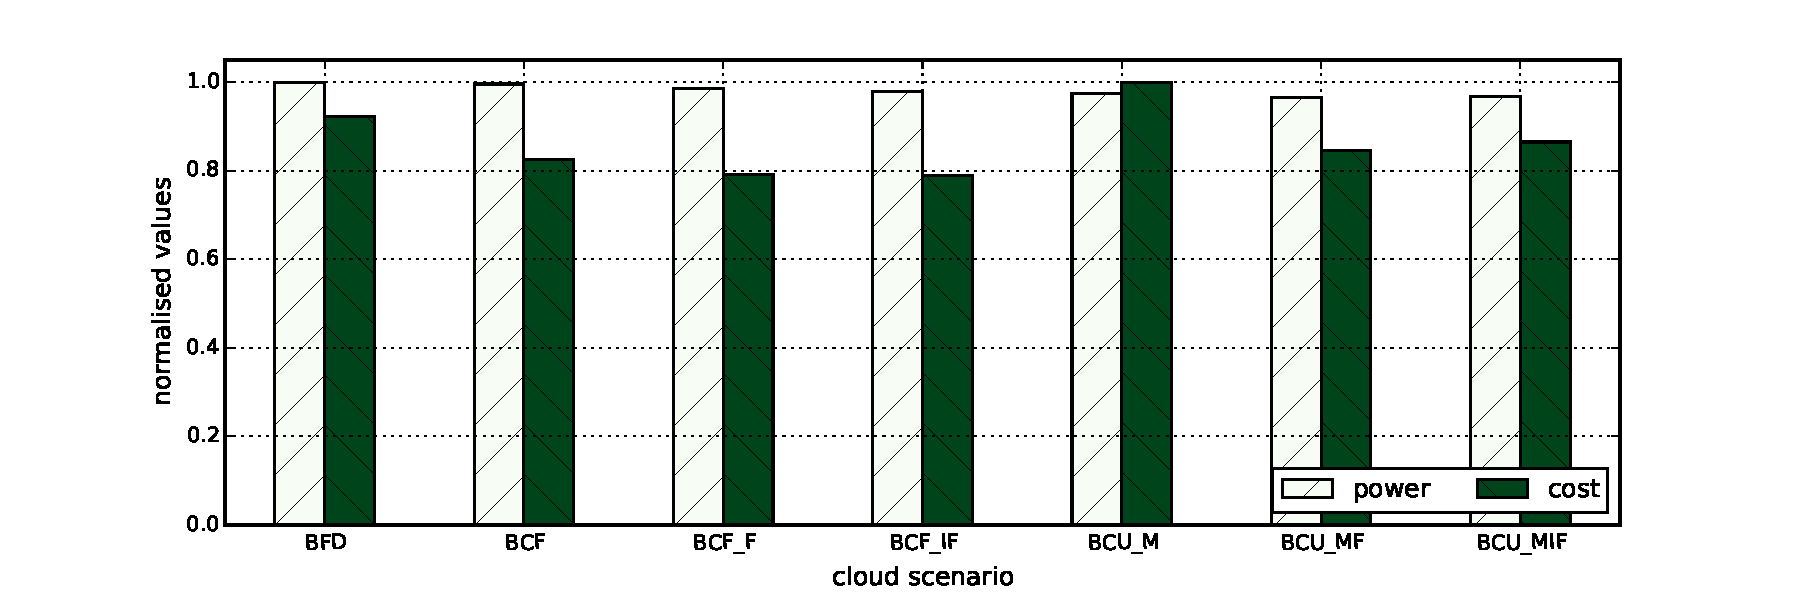
\includegraphics[width=1.00\textwidth]{figures/evaluation_and_results/energy_utility_power_vs_cost.pdf}
	\caption{Normalized cost vs power values based on the energy utility scenario}
	\label{fig:energy_utility_power_vs_cost}
\end{figure}

This graph outlines the resulting power and costs for this utility scenario across all defined schedulers (see Section \ref{sec:cloud_scheduler} for a definition of the schedulers). What can be observed is that power values differ only marginally while energy costs differ substantially. The BFD scheduler is the baseline scheduler to which all other schedulers are compared. 

For this scenario it exhibits the highest power consumption but less total costs than the BCU\_M scheduler. 

%The utility threshold for this scenario has been set to $1.8$ which 


\section{Simulation Results} \label{sec:simulation_results}

A detailed presentation of the simulator and scheduler that actually run through the simulation scenarios is given in this section. Then the results from the simulation runs based on different settings and data is presented and scenarios are compared to evaluate the most promising approach in the defined setting. Finally the results are discussed and evaluated to draw conclusions about the possible performance gains when running these scenarios, and how much they differ from the optimal solution. 

%%% final , summarized %%%




\subsection{Total costs}


\begin{table}[ht]
\centering

\begin{tabular}{lrrrrrrr}
\toprule
{} &     BFD &     BCU &   BCU\_F &  BCU\_IF &   BCU\_M &  BCU\_MF &  BCU\_MIF \\
\midrule
DA Summer &  208.36 &  181.72 &  171.85 &  174.53 &  186.19 &  \textbf{169.86} &   173.29 \\
RT Summer &  315.96 &  263.32 &  265.21 &  256.08 &  273.87 &  259.98 &   \textbf{252.09} \\
DA Spring &  930.41 &  630.13 &  592.83 &  600.42 &  625.62 &  \textbf{585.97} &   595.81 \\
RT Spring &  966.04 &  710.59 &  659.92 &  699.13 &  747.06 &  \textbf{647.57} &   668.35 \\
\bottomrule
\end{tabular}
\caption{Total costs for different scenarios (in \$)}
\end{table}

\begin{table}[ht]
\centering
\begin{tabular}{lrrrrrrr}
\toprule
{} &  BFD &    BCU &  BCU\_F &  BCU\_IF &  BCU\_M &  BCU\_MF &  BCU\_MIF \\
\midrule
DA Summer &    0 &  12.79 &  17.52 &   16.24 &  10.64 &   \textbf{18.48} &    16.83 \\
RT Summer &    0 &  16.66 &  16.06 &   18.95 &  13.32 &   17.72 &    \textbf{20.21} \\
DA Spring &    0 &  32.27 &  36.28 &   35.47 &  32.76 &   \textbf{37.02} &    35.96 \\
RT Spring &    0 &  26.44 &  31.69 &   27.63 &  22.67 &   \textbf{32.97} &    30.82 \\
\bottomrule
\end{tabular}
\caption{Normalized total cost reductions for different scenarios (in \%)}
\end{table}





